% The topic, motivation, the importance of adaptivity 
\chapter{Program Analysis for Adaptive Data Analysis}
\label{ch:adapt_intro}


Data analysts run their data analysis on sample data drawn from the population they want to study because it is usually impossible to run it on the population. The generalization error is used to measure whether the results from the sample data generalize to the population. Hence, guaranteeing a low generalization error is an important topic in the data analysis area. 

An adaptive data analysis can be seen as a process composed by multiple queries interrogating some data, where the choice of which query to run next may rely on the results of previous queries. The generalization error of each individual query/analysis can be controlled by using an array of well-established statistical techniques. However, when queries are arbitrarily composed, the different errors can propagate through the chain of different queries and result in a generalization error that is too high. To address this issue, data analysts are designing several techniques that not only guarantee the bounds on the generalization errors of single queries, but that also guarantee bounds on the generalization error of the composed analyses. 
The total number of queries and the depth of the chain of queries are of great significance when attempting to limit the generalization error when the composed data analyses are adaptive. 
The choice of which of these techniques to use often depends on the depth of the chain of queries that an adaptive data analysis can generate.   % Gap
% Unfortunately, this depth which relies on the program(implementation) itself is costly in human efforts, and how to statically obtain this information is not well studied to support data analysts.

\section{Adaptive Data Analysis}
\label{sec:adapt-backgroung}
Consider a dataset $X$ consisting of $n$ independent samples from some unknown population $\dist$.  How can we ensure that the conclusions drawn from $X$ \emph{generalizes} to the population $\dist$?  Despite decades of research in statistics and machine learning on methods for ensuring generalization, there is an increased recognition that many scientific findings generalize poorly (e.g. 
\cite{Ioannidis05,GelmanL13}
).  While there are many reasons a conclusion might fail to generalize, one that is receiving increasing attention is \emph{adaptivity}, which occurs when the choice of method for analyzing the dataset depends on previous interactions with the same dataset~\cite{GelmanL13}.

 Adaptivity can arise from many common practices, such as exploratory data analysis, using the same data set for feature selection and regression, and the re-use of datasets across research projects. Unfortunately, adaptivity invalidates these traditional methods for ensuring generalization and statistical validity, which assume the method is selected independently of the data. The misinterpretation of adaptively selected results has even been blamed for a ``statistical crisis'' in empirical science~\cite{GelmanL13}.
%  ~\cite{GelmanL13}.

\begin{figure}
    \centering
    \includegraphics[width=0.9\columnwidth]{chapters/adapt/overview-dissertation.png}
    \caption{Overview of our adaptive data analysis model. }
    \label{fig:adaptivity-model-overview}
\vspace{-0.5cm}
\end{figure}

A line of work initiated by \citet{DworkFHPRR15}, \citet{HardtU14} posed the question: Can we design \emph{general-purpose} methods that ensure generalization in the presence of adaptivity, together with guarantees on their accuracy?  The idea that has emerged in these works is to use randomization to help ensure generalization. Specifically, these works have proposed to mediate the access of an adaptive data analysis to the data by means of queries from some pre-determined family (we will consider here statistical or linear queries) that are sent to a  \emph{mechanism} which uses some randomized process to guarantee that the result of the query does not depend too much on the specific
sampled dataset. This guarantees that the results of the queries generalize well. This approach is described in Figure~\ref{fig:adaptivity-model-overview}.  We have a population that we are interested in studying, and a dataset containing individual samples from this population. The adaptive data analysis we are interested in running has access to the dataset through queries of some pre-determined family (e.g., statistical or linear queries) mediated by a mechanism. This mechanism uses randomization to reduce the generalization error of the queries issued to the data.
This line of work has identified many new algorithmic techniques for ensuring generalization in adaptive data analysis, leading to algorithms with greater statistical power than all previous approaches. Common methods proposed by these works include, the addition of noise to the result of a query, data splitting, etc. Moreover, these works have also identified problematic strategies for adaptive analysis, showing limitations on the statistical power one can hope to achieve. Subsequent works have then further extended the methods and techniques in this approach and further extended the theoretical underpinning of this approach, e.g.~\cite{dwork2015reusable,dwork2015generalization,BassilyNSSSU16,UllmanSNSS18,FeldmanS17,jung2019new,SteinkeZ20,RogersRSSTW20}.
%

A key development in this line of work is that the best method for ensuring generalization in an adaptive data analysis depends to a large extent on the number of \emph{rounds of adaptivity}, the depth of the chain of queries. As an informal example, the program $x \leftarrow q_1(D);y \leftarrow q_2(D,x);z \leftarrow q_3(D,y)$ has three rounds of adaptivity, since $q_2$  depends on $D$ not only directly because it is one of its input but also via the result of $q_1$, which is also run on $D$, and similarly,  $q_3$ depends on $D$ directly but also via the result of $q_2$, which in turn depends on the result of $q_1$. The works we discussed above showed that, not only does the analysis of the generalization error depend on the number of rounds, but knowing the number of rounds actually allows one to choose methods that lead to the smallest possible generalization error. As an example, when a study includes queries with a large number of rounds of adaptivity, then a low generalization error can be achieved by adding Gaussian noise scaled to the number of rounds to the result of each query.
When instead a study includes queries with a low number of rounds of adaptivity, then a low generalization error can be achieved by using more specialized methods, such as the reusable holdout technique from~\citet{DworkFHPRR15}. 


\subsection{Some Results in Adaptive Data Analysis}
In Adaptive Data Analysis an \emph{analyst} is interested in studying some distribution $\dist$ over some domain $\univ$.  Following previous works~\cite{DworkFHPRR15,HardtU14,BassilyNSSSU16}, we focus on the setting where the analyst is interested in answers to \emph{statistical queries} (also known as \emph{linear queries}) over the distribution.  A statistical query is usually defined by some function $\query \from \univ \to [-1,1]$ (often other codomains such as $[0,1]$ or $[-R,+R]$, for some $R$, are considered). \wq{$\mathbb{E}$ represents the expectation.} The analyst wants to learn the \emph{population mean}, which (abusing notation) is defined as $$\query(\dist) = \ex{\sample \sim \dist}{\query(\sample)}.$$

However, the distribution $\dist$ can only be accessed via a set of \emph{samples} $\sample_1,\dots,\sample_n$ drawn from $\dist$. We assume that the samples are drawn independently and identically distributed (i.i.d.).  These samples are held by a mechanism $\mech(\sample_1,\dots,\sample_n)$ who receives the query $\query$ and computes an answer 
$$\answer \approx \query(\dist).$$

The na\"ive way to approximate the population mean is to use the \emph{empirical mean}, which (abusing notation) is defined as $$\query(\sample_1,\dots,\sample_n) = \frac{1}{n} \sum_{i=1}^{n} \query(X_i).$$
However, the mechanism $M$ can then adopt some methods for improving the generalization error.

In this work, we consider analysts that ask a sequence of $\qlen$ queries $\query_1,\dots,\query_\qlen$.  If the queries are all chosen in advance, independently of the answers of each one of them, then we say they are \emph{non-adaptive}.  If the choice of each query $\query_j$ depend on the prefix $\query_1,\answer_1,\dots,\query_{j-1},\answer_{j-1}$ then they are \emph{fully adaptive}.  An important intermediate notion is \emph{$\qrounds$-round adaptive}, where the sequence can be partitioned into $\qrounds$ batches of non-adaptive queries.  Note that non-interactive queries are $1$-round and fully adaptive queries are $\qlen$ rounds.

We now review what is known about the problem of answering $r$-round adaptive queries.  
\begin{thm} 
\label{thm:nonadapt-adapt}
For any distribution $\dist$, and any $k$ \emph{non-adaptive} statistical queries, the empirical mean satisfies
$$
\max_{j=1,\dots,\qlen} | \answer_j - \query_j(\dist) | = O\left( \sqrt{\frac{\log \qlen}{n}}  \right)
$$
For any $\qrounds \geq 2$ and any \emph{$\qrounds$-round adaptive} statistical queries, it satisfies
$$
\max_{j=1,\dots,\qlen} | \answer_j - \query_j(\dist) | = O\left( \sqrt{\frac{\qlen}{n}}  \right)
$$
\end{thm}
These bounds are tight (up to constant factors) which means that even allowing one extra round of adaptivity leads to an exponential increase in the generalization error of the empirical mean, from $\log \qlen$ to $\qlen$.

\citet{DworkFHPRR15} and \citet{BassilyNSSSU16} showed that by using an alternative mechanism $M$ which uses randomization in order to limit the dependency of a single query on the specific data instance, one 
can actually achieve a much stronger generalization error as a function of the number of queries, specifically.
\begin{thm}[\cite{DworkFHPRR15, BassilyNSSSU16}] \label{thm:gaussiannoise} For any $k$, there exists a mechanism such that for any distribution $\dist$, and any $\qrounds \geq 2$ any \emph{$\qrounds$-round adaptive} statistical queries, it satisfies
$$
\max_{j=1,\dots,\qlen} | \answer_j - \query_j(\dist) | = O\left( \frac{\sqrt[4]{\qlen}}{\sqrt{n}}  \right)
$$
%And there is an analyst that make this bound tight (up to constant factors).
\end{thm}
Notice that Theorem~\ref{thm:gaussiannoise} has different quantification in that the optimal choice of the mechanism depends on the number of queries.  Thus, we need to know the number of queries \emph{a priori} to choose the best mechanism.
% \footnote{ \label{fn1} One can, in principle, avoid knowing the number of queries and rounds \emph{a priori} using a ``guess-and-double'' strategy, however this would weaken the bound on generalization error considerably.}


%Later work by Dwork 
% \etal~\cite{??} 
\citet{DworkFHPRR15}
also gave more refined bounds in terms of the number of rounds of adaptivity.   %\footnotemark[\ref{fn1}] 
%Specifically, 
\begin{thm}[\cite{DworkFHPRR15}] \label{thm:gaussiannoise2} For any $r$ and $k$, there exists a mechanism such that for any distribution $\dist$, and any $\qrounds \geq 2$ any \emph{$\qrounds$-round adaptive} statistical queries, it satisfies
$$
\max_{j=1,\dots,\qlen} | \answer_j - \query_j(\dist) | = O\left( \frac{r \sqrt{\log k}}{\sqrt{n}}  \right)
$$
%And there is an analyst that make this bound tight (up to constant factors).
\end{thm}

This suggests that if one knows a good \emph{a priori upper bound on the number of rounds of adaptivity}, one can get a much better guarantee of the generalization error, but only by using an appropriate choice of the mechanism.




%gap
This scenario motivates us to explore the design of program analysis techniques that can be used to estimate the number of \emph{rounds of adaptivity} that a program implementing a data analysis can perform. These techniques could be ultimately be integrated into a tool for adaptive data analysis such as the \emph{Guess and Check} framework by~\citet{RogersRSSTW20}. 
%

\section{Challenges and Our solutions }
\label{sec:adapt-challenges}

\subsection{Formalizing an Adaptive Data Analysis Model}
\label{subsec:adapt-formalizing-model}
The first problem we face is \emph{how to define formally} a model for adaptive data analysis which is general enough to support the methods we discussed above and would permit to formulate the notion of adaptivity these methods use. We take the approach of designing a programming framework for submitting queries to some \emph{mechanism} giving access to the data mediated by one of the techniques we mentioned before, e.g., adding Gaussian noise, randomly selecting a subset of the data, using the reusable holdout technique, etc. In this approach, a program models an \emph{analyst} asking a sequence of queries to the mechanism. The mechanism runs the queries on the data applying one of the methods discussed above and returns the result to the program. The program can then use this result to decide which query to run next. Overall, we are interested in controlling the generalization of the results of the queries which are returned by the mechanism, by means of the adaptivity. 

To define adaptivity we consider a dependency graph between the different queries that we synthesize from the possible execution traces of the program representing the data analysis. The dependency graph is built by inspecting all the possible traces of execution and by identifying situations where the execution of a query \emph{causes} the execution of another query. Intuitively, a query $Q$ may depend on another query $P$, if there are two values that $P$ can return which affect in different ways the execution of $Q$. 
For example, as depicted in \cite{dwork2015reusable}, a machine learning algorithm for constructing a classifier can be modeled by first computing each feature's correlations with the label via a sequence of queries and then constructing the classifier based on the correlation values. If one feature's correlation changes, the classifier depending on features is also affected.  
This notion of dependency builds on the execution trace as a \emph{causal history}. In particular, we are interested in the history or provenance of a query up until this is executed, we are not then concerned about how the result is used --- except for tracking whether the result of the query may further cause some other query. This is because we focus on the generalization error of queries and not their post-processing.  

\paragraph{Through an Example}
 We motivate the definition of adaptivity we will use through a simple example illustrated in Figure~\ref{fig:simpl-two-round-graph}(a), which implements a simple "two rounds strategy".

%
% Figure~\ref{fig:simpl-two-round-graph}.  
{
\begin{figure}
%\begin{equation*}
%\label{}
% \[
%TR(k) \triangleq
%{
\centering
\begin{subfigure}{.2\textwidth}
\begin{centering}
$
\begin{array}{l}
   a \leftarrow 0; \\
   i \leftarrow 0 ; \\
    \eloop ~ 3 ~ \edo ~ \\
    \quad
     x \leftarrow q_1(\chi[i])   ; \\
    \quad a \leftarrow a+x; \\
        \quad i \leftarrow i+1; \\
    l \leftarrow q_2(\chi[4]*a)\\
\end{array}
$
\caption{}
\end{centering}
\end{subfigure}
%}
\quad
\begin{subfigure}{.2\textwidth}
\begin{centering}
$
\begin{array}{l}
   \clabel{ a \leftarrow 0}^{1}; \\
   \clabel{ i \leftarrow 0}^{2} ; \\
    \eloop ~ \clabel{3}^{3} ~ \edo ~ \\
    \quad
    \clabel{ x \leftarrow q_1(\chi[i])}^{4}   ; \\
    \quad \clabel{a \leftarrow a+x}^{5}; \\
        \quad \clabel{i \leftarrow i+1}^{6}; \\
    \clabel{l \leftarrow q_2(\chi[4]*a)}^{7}\\
\end{array}
$
\caption{}
\end{centering}
\end{subfigure}
\begin{subfigure}{.55\textwidth}
%}
\qquad
\begin{centering}
$\vcenter{\hbox{
% \]
% \begin{wrapfigure}{R}{0.5\textwidth}
% \begin{figure}
% \begin{tcolorbox}[colback=white]
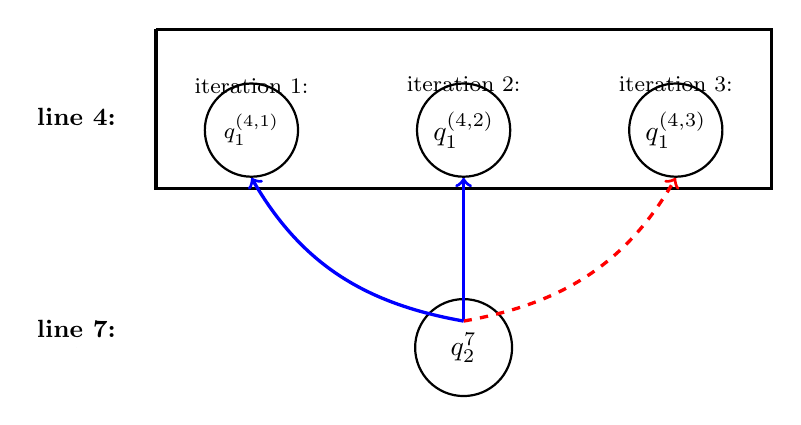
\begin{tikzpicture}[scale=\textwidth/18cm,samples=200]
%%% The nodes represents the k query in the first round
\draw[very thick] (0.2,6)  -- (11.8,6) -- (11.8,3) -- (0.2,3) -- (0.2,6);
\draw[black] (-1.3, 4) circle (0pt) node [anchor=south]{\small{\textbf{line 4:}}};
\filldraw[black] (-1.3, 0) circle (0pt) node [anchor=south]{\small{\textbf{line 7:}}};
%
\draw[thick] (2, 4.1) circle (25pt) 
node[label={above: \footnotesize{iteration 1:}}] {\footnotesize{$q_1^{(4,1)}$}} ;
\draw[thick] (6, 4.1) circle (25pt) node[label={[black]above: \footnotesize{iteration 2:}}] 
{$q_1^{(4,2)}$};
\draw[thick] (10, 4.1) circle (25pt) node [label={[black]above: \footnotesize{iteration 3:}}]
{$q_1^{(4,3)}$};
\draw[thick] (6, 0) circle (26pt) node {$q_2^7$};
\draw[very thick,->, blue] (6, 0.5)  -- (6, 3.2) ;
\draw[very thick,->, red, dashed] (6, 0.5)  to [out=10,in=240] (10, 3.2) ;
\draw[very thick,->, blue] (6, 0.5)  to [out=170,in=300]  (2, 3.2) ;
\end{tikzpicture}
}
}
$
\caption{}
\end{centering}
\end{subfigure}
% \end{wrapfigure}
% \end{equation*}
\vspace{-0.4cm}
 \caption{(a) Example of a program with two rounds of adaptivity, (b) Labeled program for the same example, (c) The corresponding query-based dependency graph.}
\label{fig:simpl-two-round-graph}
\vspace{-0.5cm}
\end{figure}
}
 %
 %
% \mg{I don't think the example is good enough. Specifically, I think that we should use the rows of the database somewhere, we don't use them at all in the example. Also, do we have bounds that depend on a variable? I thought we had only loops with constants. I sketched something that could work for us.}

In this example, the analyst asks queries to the mechanism in two phases. In the first phase,  the analyst asks a fixed number $k$ of queries (in the example $k=3$) and stores the answers that are provided by the mechanism. In the second phase, the analyst constructs a new query based on the results of the previous $k$ queries and sends this query to the mechanism. More specifically, we assume that, in this example, the domain $X$ contains at least four numeric attributes, which we index just by natural numbers. The queries inside the loop correspond to the first phase and compute an approximation of the empirical mean of the first three attributes. The query outside the loop corresponds to the second phase and computes an approximation of the empirical mean where each record is weighted by the sum of the empirical mean of the first three attributes. 
%
Queries are of the form $q(e_q)$ where $e_q$ is a query expression with a special variable $\chi$ representing a possible row. Mainly $e_q$ represents a function from $X$ to some domain $U$, for example $U$ could be $[-1,1]$ or $[0,1]$. This function characterizes the linear query we are interested in running. As an example, $x \leftarrow q(\chi[2])$ computes an approximation, according to the used mechanism, of the empirical mean of the second attribute, identified by $\chi[2]$. Notice that we don't materialize the mechanism but we assume that it is implicitly run when we execute the query.  

% a predicate  (the sum in this example). The program in the {\tt Loop} language implementing this algorithm is presented in Figure~\ref{fig:simpl-two-round-graph}(a). The answers in the first round are accumulated in variable $a$. The index $i$ is a loop counter used to express $k$(we pick $k=3$) queries $q_1(\chi[i])$ of the first round. The query $q_2(\chi[4]+a)$ in the second round uses $a$.} 

 In order to analyze programs like the one we just discussed, it is convenient to work with a version of the program where similar commands can be easily distinguished. For this reason, we use labeled versions of programs, where labels correspond to lines of code. As an example, we give the labeled version of the two rounds example program in Figure~\ref{fig:simpl-two-round-graph}(b).
%  We leave
%  more details about the labeled {\tt Loop} language in Section~\ref{sec:loop_language}. 
%  When we try to analyze this program, we run quickly into the issue that queries of the form $q(e)$ can be run multiple times with different values for $e$ since variables can be reassigned. To identify variables For instance, look at aforementioned program of two round strategy, variable $a$ used at line $7$ comes from the assignment at line $5$ instead of line $1$. To avoid this confusion, we add line numbers(we call it label) to commands. The labelled one is shown in Figure~\ref{fig:simpl-two-round-graph}(b).
%  We leave
%  more details about the labelled {\tt Loop} language in Section~\ref{sec:loop_language}. 

% Our framework aims to provides an upper bound on the number of rounds of adaptivity (or the depth of chain of queries connected by dependency relation), denoted as $A$ in the Fig~\ref{fig:structure}, of a high level program $P$. We will go through one concrete example called "two rounds algorithm"  after the brief introduction of high level loop language, in which the target program ($TR^{H}$) implementing "two rounds algorithm" is written.

% In the high level loop language, the assignment command $x \leftarrow e$ and the loop command $\eloop ~ \aexpr  ~ \edo ~ c $ is standard. The command $ \assign{x} {q(\expr)}$ stores the result of a query $q(\expr)$ in which the elements used to construct the query are presented by the expression $\expr$. 
% We have the standard arithmatic operators denoted as $\opuls_a$, boolean operators as $\oplus_b$, and relational operators as $*_r$. 
% \[
% \begin{array}{llll}
% %  \mbox{Arithmatic Operators} & *_a & ::= & + ~|~ - ~|~ \times 
% % %
% % ~|~ \div \\  
% %   \mbox{Boolean Operators} & *_b & ::= & \lor ~|~ \land ~|~ \neg\\
% %   %
% %   \mbox{Relational Operators} & *_r & ::= & < ~|~ \leq ~|~ = \\  
% \mbox{AExpr} & \aexpr & ::= & 
% 	n ~|~ x ~|~ \aexpr *_a \aexpr ~|~ {[] ~|~ [\aexpr_0, \dots, \aexpr_i]  }  \\
% \mbox{BExpr} & \bexpr & ::= & 
% 	\etrue ~|~ \efalse  ~|~ \neg \bexpr
% 	 ~|~ \bexpr *_b \bexpr
% 	~|~ \aexpr *_r \aexpr \\
% \mbox{Command} & c & ::= &   \assign{x}{\expr} ~|~  \assign{x} {q(\expr)} ~|~  c ; c ~|~ \eif(\bexpr, c_1, c_2) 
% 	 ~|~ \eskip \sep {\eloop ~ \aexpr  ~ \edo ~ c }
% \end{array}
% \]

This example is intuitively 2-rounds adaptive. The reason is that we have two distinguished phases and the queries that we ask in the first phase do not depend on each other, while the last query depends on all the previous queries. 
However, capturing this concept formally is surprisingly difficult. The difficulty comes from the fact that a query can depend on the result of another query in multiple ways, by means of data dependency or control flow dependency. In order to find the right definition for our goal, we take inspiration from the known results of the data analysis model we discussed above. This theory tells us that what we want to measure is the generalization error on the result of a query and not an arbitrary manipulation of the query. Indeed, arbitrary manipulations can change the generalization error. As an example, suppose that $v$ is the result we get from running a query, if we multiply this result by some constant, we are also changing the incurred error. Moreover, this theory tells us that we can always consider a non-adaptive set of queries as to being adaptive, and more importantly, that we can transform an adaptive query into a non-adaptive one, incurring an exponential blow-up of the number of queries. For example, we could ask many queries upfront, and depending on the results of some of them, we could return the results of others. For these reasons, we define adaptivity in terms of the possible execution traces of the program on all possible inputs. A trace of execution is a list of query requests of the form $[q(v_1)^{(l_1,w_1)},\ldots, q(v_n)^{(l_n,w_n)}]$, where every occurrence of a query is labeled with the line of code $l$ it appears at, and the counter $w$ identifying the possible loop iteration happening when a query is called. For example, in $q(v_1)^{(3,1)}$, the superscript $(3,1)$ indicates that the query is asked at line $3$ and that the query is requested in the first iteration of the loop. When the query is not in a loop, we omit the counter.

Using traces we can identify situations when one query can affect the execution of another one. Using this information we can build a directed graph, called the query-based dependency graph, where the nodes represent the queries that are executed and the edges between two nodes represent the fact that one query may depend on the other. We show such a graph for our running example in Figure~\ref{fig:simpl-two-round-graph}(c). We can then define adaptivity as the longest possible path in this graph.  Looking again at our example, it is easy to see that the longest path in the graph in Figure~\ref{fig:simpl-two-round-graph}(c), which we mark with a red dashed arrow, is $2$, as we were expecting.

% \wq{
%  Now that we we look at the adaptivity of this example. First of all, to apply the theorems described above, the adaptivity is achieved in the setting that the analyst is only interested in the answers to the sequence of linear queries he/she asks to the mechanism. So the adaptivity of this two round strategy can be obtained by finding out a sequence of adaptively chosen queries with longest length, among all the queries the analyst asks. Intuitively, this longest sequence of adaptively chosen queries can be transformed to, the longest path in a directed graph where the node representing the queries asked and the edge between two nodes standing for one query may depend on the other. We show such a graph in Figure~\ref{fig:simpl-two-round-graph}(c), and call it, query-based dependency graph. In the graph, every node stands for a query with annotation. 
% }
% \wq{To draw the query-based dependency graph, we need to consider two components: the vertices and the edges. Our approach is defined as follows. 
% \begin{enumerate}
%     \item The vertices are collected by a trace-based operational semantics, which tracks the execution of the program.
%     \item The edges are defined by a formal definition of may-dependency between two queries.
% \end{enumerate}
% }
  % trace operation semantics
%   The trace-based operational semantics of the loop language have the shape of $\config{m, c, t,w} \xrightarrow{} \config{m', c',  t', w'}  $. It works on a configuration of memory $m$, a program $c$, a trace $t$, a loop map $w$. The trace $t$ is a list of annotated queries. One annotated query is a  
%   query with the annotation $(l,w)$, $l$ is the line number and $w$ is used for loop and tells the iteration number. For example, the 
%   query $q()$ at line $3$ in the example $TR$ at the first iteration is represented as the annotated query $q()^{(3, [2:1])}$. The loop map $w$ is a map, from the line number of the loop counter ( $\clabel{k}^{2}$ ) to its iteration number. The trace tracks the query asked during the execution, still use the $TR$ as an example. The trace of $TR$ starting with an empty loop map $\emptyset$ has the following trace $t_{tr}$, supposing $k=3$. 
%   \[t_{tr} = [q()^{(3,[2:1])},q()^{(3,[2:2])},q()^{(3,[2:3])}, q(a)^{(5,\emptyset)}  ] \]
  
% % define rounds of adaptivity
% The second component is the defintion of may-dependency between queries. In particular, what we need to be clear is what does it mean by saying one query may depend on another query. To this end, we look at trace.  Now whether one query $q$ depends on another query $p$ can be checked, by witnessing $q$ in the new generated trace upon change of $p$. For example, if we change the result of $q()^{(3,[2:1])}$, we have a new trace $t'_{tr}$, and $a$ may change as well. In this case, $q(a)^{(5, \emptyset)}$ may not show up in the new generated trace $t'_{tr}$. So we think $q(a)^{(5, \emptyset)}$ may depend on $q()^{(3,[2:1])}$. 
% trace based dependency relation is challenging

\begin{figure}
    \centering    
    \begin{tikzpicture}
    % {node distance = 2cm, auto}
  % nodes
%   \node[block] at (2,-6) (block6) {$f_6$};
  \node [block][text width=8em](high){ Program $P$ } ;
  \node [block, right of = high, node distance = 7cm, text width=13em](ssa){SSA Program $P^{s}$} ;
  \node [block, below of = ssa, node distance = 2cm, text width=13em] (bound) {Estimated Adaptivity $Adapt$} ;
  \node [block, below of = high, node distance = 2cm, text width=8em](adapthigh){Adaptivity $A$};
  % edges
  \path [line, thick] (high) -- node [above] {transformation} (ssa) ;
  \path [line, thick] (ssa) -- node [label={[label distance=.2cm]0:\ADAPTSYSTEM}] {} (bound);
  \path [line, thick] (bound) -- node [below] {upper bound} (adapthigh);
  \path [line, thick]  (high) -- node [label={[label distance=-3cm]0:trace-based graph}]{}(adapthigh);   
 \end{tikzpicture} 
   \caption{High level architecture of {\ADAPTSYSTEM}.}
    \label{fig:structure}
\end{figure}


\subsection{Static Analysis for Adaptivity}

The second problem we face is \emph{how to estimate the adaptivity of a given program}. The adaptive data analysis model we consider and our definition of adaptivity suggest that for this task we can use a  program analysis that is reminiscent of information flow control. However, this is not sufficient since, in general, a query $Q$ is not a monolithic block but rather it may depend, through the use of variables and values, on other parts of the program. Hence, we also need to consider some form of data-flow analysis. Our program analysis, named {\ADAPTSYSTEM}, combines information flow and data-flow analysis using an adjacency matrix $M$ representing the dependency between different variables, and a vector $V$ representing different queries. These two components allow us to over-approximate the dependency graph and estimate the adaptivity of the program. 

To simplify our analysis, we do not directly apply the program analysis to the source program. Instead, we first transform the program into static single assignment form, SSA form. In this form all the variables are assigned once, including variables in loops, and this helps our analysis in avoiding the complexity of handling variables reassignment. Moreover, we show that by analyzing programs in SSA form, we get a bound on the number of rounds of adaptivity that is also a bound for the source program.

The high-level architecture of our static analysis framework is shown in 
 Figure~\ref{fig:structure}. The input of the analysis is a labeled program P for which the adaptivity A is defined by means of a trace-based definition, as discussed above. In order to estimate an upper bound on A, our program analysis first transforms the program P into the static single assignment (SSA) form. The goal of this step is to guarantee that each variable is assigned only once. We show the result of this transformation applied to our two rounds strategy example in Figure~\ref{fig:ssa_tworound}(a). 
 This transformation, when applied to a loop, introduces some extra variables that serve as intermediate storage. For example, in~\ref{fig:ssa_tworound}(a) there is a new instruction $[(i_3,i_1,i_2),(a_3,a_1,a_2)]$ after the loop. This instruction asserts that the value of the new variables $i_3$ and $a_3$, depending on the execution step, may come from $i_1$ or $i_2$, $a_1$ or $a_2$, respectively. \wq{To be concrete, if it is in the first iteration of the loop, $i_3 = i_1$, otherwise, $i_3 = i_2$.} For those readers who are familiar with SSA, it can be regarded as another form of the phi node. The transformation of a program into SSA form preserves the execution traces, and so, in turns, it preserves the adaptivity. 

\begin{figure} 
\centering
   \begin{subfigure}{.2\textwidth}
   \begin{centering}
   $
   \begin{array}{l}
  \clabel{ a_1 \leftarrow 0}^{1}; \\
   \clabel{ i_1 \leftarrow 0}^{2} ; \\
    \eloop ~ \clabel{3}^{3} ~ \edo ~ \\ 
    \quad [(i_3, i_1,i_2), (a_3,a_2,a_1)] \\
    %  \quad i_3 = \phi(i_1,i_2); \\
    %   \quad a_3 = \phi(a_1,a_2); \\
    \quad
    \clabel{ x_1 \leftarrow q_1(\chi[i_3])}^{4}   ; \\
    \quad \clabel{a_2 \leftarrow a_3+x_1}^{5}; \\
        \quad \clabel{i_2 \leftarrow i_3+1}^{6}; \\
    \clabel{l_1 \leftarrow q_2(\chi[4]*a_3)}^{7}\\
    \end{array}
% {
% \begin{array}{l}
%   \clabel{ a_1 \leftarrow [] }^{1}; \\
%     \eloop ~ \clabel{k}^{2} ~ \edo ~ \\
%     \Big(
%       a_3 = \phi(a_1,a_2); \\
%      \clabel{x_1 \leftarrow q() }^{3}  ; \\
%     \clabel{a_2 \leftarrow x :: a_3}^{4}      \Big); \\
%     \clabel{l_1 \leftarrow q(a_3)}^{5}\\
% \end{array}
% }
 $
 \caption{}
   \end{centering}
   \end{subfigure}
   \begin{subfigure}{.5\textwidth}
   \begin{centering}
   $\vcenter{\hbox{
% \]
% \begin{wrapfigure}{R}{0.5\textwidth}
% \begin{figure}
% \begin{tcolorbox}[colback=white]
   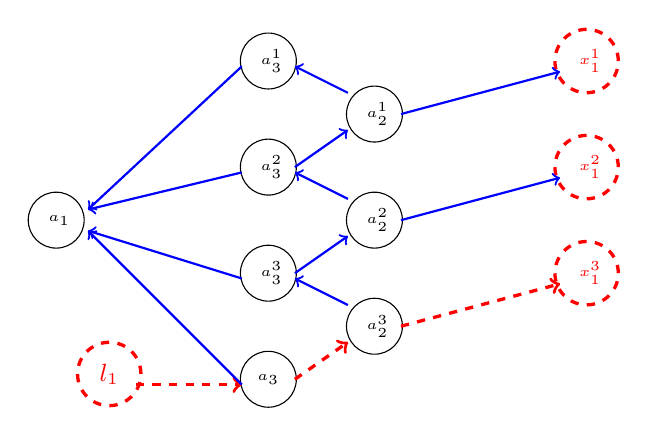
\begin{tikzpicture}[scale=\textwidth/18cm,samples=200]
%%% The nodes represents the k query in the first round
% \draw[very thick] (-1,6)  -- (13,6) -- (13,3) -- (-1,3) -- (-1,6);
% \draw[black] (-2.5, 4) circle (0pt) node [anchor=south]{\textbf{line 4:}};
% \draw[thick] (1, 1.1) circle (25pt) node
% % node[label={above: \small{iteration 1:}}] 
% {\tiny{$q_1^{(5,1)}$}} ;
\draw[] (2, 5.1) circle (15pt) node
{\tiny{ $a_1$}};
\draw[] (6, 8.1) circle (15pt) node
{\tiny{ $a_3^{1}$}};
% \draw[thick] (8, 11.1) circle (15pt) node
% {\tiny{ $x_{1}^{1}$}};
% \draw[thick] (10, 10.1) circle (15pt) node
% {\tiny{ $x_{2}^{1}$}};
\draw[very thick, dashed, red] (12, 8.1) circle (17pt) node{\tiny{\textbf{ $x_{1}^{1}$}}};
\draw[] (8, 7.1) circle (15pt) node
{\tiny{ $a_{2}^{1}$}};
\draw[] (6, 6.1) circle (15pt) node{\tiny{ $a_3^{2}$}};
% \draw[thick] (10, 8.1) circle (15pt) node
% {\tiny{ $x_{1}^{2}$}};
% \draw[thick] (12, 7.1) circle (15pt) node
% {\tiny{ $x_{2}^{2}$}};
\draw[very thick, dashed, red] (12, 6.1) circle (17pt) node{\tiny{\textbf{ $x_{1}^{2}$}}};
\draw[] (8, 5.1) circle (15pt) node
{\tiny{ $a_{2}^{2}$}};
% \draw[thick] (12, 5.1) circle (15pt) node
% {\tiny{ $x_1^{3}$}};
\draw[] (6, 4.1) circle (15pt) node
{\tiny{ $a_3^{3}$}};
\draw[very thick, dashed, red] (12, 4.1) circle (17pt) node{\tiny{\textbf{ $x_1^{3}$}}};
% \draw[thick] (12, 3.1) circle (15pt) node
% {\tiny{ $x_2^{3}$}};
\draw[] (8, 3.1) circle (15pt) node
{\tiny{ $a_{2}^{3}$}};
 \draw[] (6, 2.1) circle (15pt) node 
{\tiny{$a_3$}};
% \filldraw[black] (-2.5, 0) circle (0pt) node [anchor=south]{\textbf{line 7:}};
\draw[very thick, dashed, red] (3, 2.2) circle (17pt) node {\small{\textbf{$l_1$}}};
%dotted
 \draw[->, red, very thick, dashed] 
         (3.5, 2)  -- (5.5, 2) ;
%   \draw[->, red, very thick,snake=snake, segment amplitude=.4mm,
%          segment length=2mm, line after snake=1mm] 
%          (6, 0.5)  -- (6, 1.6) ;
\draw[->, red, very thick, dashed](6.5, 2.1)  -- (7.5, 2.8) ;
 \draw[->, red, very thick, dashed] (8.5, 3.1)  -- (11.5, 3.9) ;
    \draw[thick,->, blue] (8.5, 5.1)  -- (11.5, 5.9) ;
\draw[thick,->, blue] (8.5, 7.1)  -- (11.5, 7.9) ;
%  \draw[thick,->, blue] (10.5, 4.1)  -- (11.5, 4.8) ;
%   \draw[thick,->, red] (10.5, 4.1)  -- (11.5, 3.3) ;
   \draw[thick,->, blue] (7.5, 3.5)  -- (6.5, 4.0) ;
   \draw[thick,->, blue] (6.5, 4.1)  -- (7.5, 4.8) ;
    %  \draw[thick,->, blue] (10.5, 6.1)  -- (11.5, 6.8) ;
% \draw[thick,->, blue] (10, 6.6)  -- (10, 7.6) ;
\draw[thick,->, blue] (7.5, 5.5)  -- (6.5, 6.0) ;
 \draw[thick,->, blue] (6.5, 6.1)  -- (7.5, 6.8) ;
% \draw[thick,->, blue] (8.5, 9.1)  -- (9.5 , 9.8) ;
% \draw[thick,->, blue] (8, 9.6)  -- (8, 10.6) ;
\draw[thick,->, blue] (7.5, 7.5)  -- (6.5, 8.0) ;
\draw[thick,->, blue] (5.5, 8.0)  -- (2.6, 5.3) ;
\draw[thick,->, blue] (5.5, 6.0)  -- (2.6, 5.3) ;
\draw[thick,->, blue] (5.5, 4.0)  -- (2.6, 4.9) ;
\draw[thick,->, blue] (5.5, 2.0)  -- (2.6, 4.9) ;
% \draw[very thick,->, red] (6, 0.5)  to [out=30,in=240] (11, 3.2) ;
% \draw[very thick,->, blue] (6, 0.5)  to [out=150,in=300]  (1, 3.2) ;
\end{tikzpicture}
}
}
$
\caption{}
   \end{centering}
   \end{subfigure}
    \vspace{-0.3cm}
    \caption{(a) Example of a SSA program with two rounds of adaptivity (b) The corresponding variable-based dependency graph.}
    \vspace{-0.5cm}
    \label{fig:ssa_tworound}
\end{figure}
%

The main component of our framework is an algorithm, which we call ${\ADAPTSYSTEM}$. This algorithm constructs a variable-based weighted directed dependency graph where nodes are annotated variables and edges represent potential dependencies between the variables. We show the variable-based dependency graph for our running two rounds example in Figure~\ref{fig:ssa_tworound}(b). The algorithm builds this dependency graph by traversing the SSA program P$^S$ and collecting the information about dependencies between the different variables in an adjacency matrix $M$, and information about the relations between queries and variables in a vector $V$. The matrix $M$ collects information about both data dependency and control flow dependency. The vector $V$ is used to assign a weight to the different nodes. In particular, to each variable related to a query, the algorithm assigns weight $1$ and to any other variables, the algorithm assigns no weight. The estimated upper bound for the adaptivity is the weight of the path in the graph with maximal weight.  \wq{In Figure~\ref{fig:ssa_tworound}(b), we have a dependency graph between variables. The nodes are the assigned variables and the edge between two nodes means one variable may have data dependency or control flow dependency(or both) on the other variable. Only the variable $x$ which is assigned with the query result via $\assign{x}{q(e_q)}$ will be marked as the weighted node with the unit weight. The nodes in a dashed circle are those special nodes associated with query requests. We want to find the path in the graph with the highest weights (the most special nodes). } The path with maximal weight is the dashed one in the graph. The weight of this path is $2$, providing us a tight upper bound on the adaptivity of P. More in general, we prove that the upper bound estimated by {\ADAPTSYSTEM} gives a sound overapproximation of the adaptivity of the analyzed program. 

% \wq{According to the aforementioned work for ensuring generalization in adaptive data analysis, the tight generalization error bound is achieved under the analyst-mechanism assumption that, the analyzed program is modelled as a procedure of an \emph{analyst} asking a sequence of queries to some mechanism and only the responded answers are back to the {analyst}, with no processing of the query results revealed. Then The adaptivtity notion under this assumption, only focusing on the queries, is the length of a sequence of adaptively chosen queries among the queries asked by the {analyst}.}
% This requires us to define  Since most of these techniques we focus in this work on queries that can be executed \emph{row-by-row}, those submitted 
% queries are specified by some function of a row in the framework.
% and how to integrate the techniques mentioned before in a programming . Hence, as a first step we Nevertheless, the corresponding study on static analysis over programs implementing adaptive analysis is not well explored, even the formal definition of this \emph{rounds of adaptivity} is not clear. Our goal is to study adaptivity and conduct analysis over programs to find the number of rounds.
% our innovation

% Based on this framework, we define adaptivity as a property based on multiple traces of executions, or in other terms as an hyperproperty~\cite{clarkson2010hyperproperties}. \wq{For the sequence of adaptively chosen queries described before, the concept of one query may depend on its previous queries and answers is necessary. } Intuitively, a query $Q$ may depend on another query $P$, if there are two 
% values that $P$ can return which affect in different ways the execution of $Q$. 
% This definition suggests that we need to consider a program analysis which is a reminiscence of information flow control. However, this is not sufficient since, in general, a query is not a monolithic block $Q$ but rather some syntactic construction depending on some expression that depends on some variables. Hence, we also need to consider some data-flow analysis. 
% In a word, what we want is a program analysis which statically provides an upper bound on the number of rounds of adaptivity, and on the number of queries that are run by programs implementing adaptive data analysis. 

% The first question we need to decide on is what language the target programs to be analyzed are written, in a functional programming language or an imperative one?     
% the reason we do not use functional programming language, 
 %We choose the imperative programming language, then the following question is what does this imperative language look like? 
%  A principle of the ideal language in our mind is supposed to be simple enough to alleviate the burden of analysis on complex components that is unnecessary to adpativity, and expressive enough to support most of the adaptive data analysis algorithms. With this principle in mind, we introduce an imperative language called the {\tt Loop} language, with one finite loop construct, allowing data analysts recursively request queries in their programs. The query request is also supported in the language.

% The query request is abstract in the loop language and shows up as a primitive construct $q(e)$, where the argument $e$ is an expression tracking the necessary information needed to construct the unique query. We choose to make query abstract for the reason that we only care about the elements(the arguments) used to construct the query instead the detail of the query, with respect to what we are interested in: whether some queries rely on some other queries.        

%  For the number of rounds of adaptivity of program in the loop language, a definition of "one query relies on another query", or "one query may depend on the other" is the next big thing. We choose to define this "may-dependency" with the help of a trace-based operational semantics.  
% %  the change of the results of the query will affect the appearance of the other in a trace of the execution. The trace is
%  The trace is a list of queries generated along with the execution of the program, a history of the execution only caring about query requests.
%  which is specified in the operational semantics and will be discussed later.


% one is the transformation of programs of the aforementioned loop language we call it "high level language", to its variant "low level language", in which the arguments of queries go into the control flow of the program. Performing such a transformation helps us to better focus on the dependency between queries because we can treat queries simply as primitive symbols in the low level loop language without worrying about the arguments of the queries affecting the results. 
% In a word, the key idea of this transformation guarantees all the effect on queries comes from the structure of the programs. 
% The other is the transformation from the "low level" programs
% to construct a dependency graph between these unique variables, and hence predict the rounds of adaptivity from the graph. To generate the dependency graph, 
% To be more specific, our framework is equipped with algorithms to record the necessary information and construct a dependency graph to reach a final estimation of the adaptivity.
\section{Contributions of {\ADAPTSYSTEM}}
\label{sec:adapt-contributions}
To Summarize, our work aims at the design of a static analysis for programs implementing adaptive analysis that can estimate their rounds of adaptivity. Specifically, our contributions are as follows:
\begin{enumerate}
    \item A programming framework for adaptive data analyses where the program represents an analyst that can query a generalization-preserving mechanism mediating the access to some data. 
    % \item A trace-based operational semantics for the loop language, specific to dependency between queries.
    \item A formal definition of the notion of adaptivity under the aforementioned analyst-mechanism model. This definition is built on a query-based dependency graph built out of all the possible program execution traces.
    % \item A transformation between the {\tt Loop} language and the ssa language, with the soundness of the transformation.
    \item A program analysis algorithm {\ADAPTSYSTEM} which provides an estimated upper bound on the adaptivity via a variable-based dependency graph.
    \item A soundness proof of the program analysis showing that the adaptivity estimated by {\ADAPTSYSTEM} bounds the true adaptivity of the program. 
\end{enumerate}



